\documentclass[12pt]{article}

\usepackage{listings}
\usepackage{cite}
\usepackage{graphicx}
\usepackage{booktabs}
\usepackage{color}
\usepackage{indentfirst}
 
\definecolor{codegreen}{rgb}{0,0.6,0}
\definecolor{codegray}{rgb}{0.5,0.5,0.5}
\definecolor{codepurple}{rgb}{0.58,0,0.82}
\definecolor{backcolour}{rgb}{0.95,0.95,0.92}
\definecolor{codeblue}{rgb}{0.7,0.8,0.215}
 
\lstdefinestyle{newStyle}{
    backgroundcolor=\color{backcolour},   
    commentstyle=\color{codegreen},
    keywordstyle=\color{blue},
    numberstyle=\tiny\color{codegray},
    stringstyle=\color{codepurple},
    basicstyle=\footnotesize,
    breakatwhitespace=false,         
    breaklines=true,                 
    captionpos=b,                    
    keepspaces=true,                 
    numbers=left,                    
    numbersep=5pt,                  
    showspaces=false,                
    showstringspaces=false,
    showtabs=false,                  
    tabsize=2
}
 
\lstset{style=newstyle}
\setcounter{section}{-1}
\usepackage[left=2cm,right=2cm,
    top=2cm,bottom=2cm,bindingoffset=0cm]{geometry}

\title{SOEN 6611 \\ SOFTWARE MEASUREMENT \\ Deliverable 1 \\
(DESCRIPTIVE-STATISTICS)}
\date{SUMMER 2018}     
\author{(Team F)\\ 
Mehak Jot Kaur\\
Roopamdeep Kaur\\
Sukhmeet Kaur\\
Amandeep Kaur Khosa\\
Kritika Kritika\\
Dmitry Kryukov
}
%\setcounter{secnumdepth}{0}
\newcommand\tabularhead[1]{
\begin{table}[h]
  \caption{Use case - #1}
  \begin{tabular}{|p{0.35\linewidth}|p{0.65\linewidth}|}
    \hline
    \textbf{Use case name} & \textbf{#1} \\
    \hline}

  \newcommand\addrow[2]{#1 &#2\\ \hline}
  
  \newcommand\adddoublerow[2]{\begin{minipage}[t][][t]{2.5cm}#1\end{minipage}%
    &\begin{minipage}[t][][t]{\linewidth}
     \begin{itemize}\setlength{\itemsep}{0pt}%
        #2     
     \end{itemize}
     \end{minipage}\\ \hline}
  
  \newcommand\addmulrow[2]{ \begin{minipage}[t][][t]{2.5cm}#1\end{minipage}% 
     &\begin{minipage}[t][][t]{\linewidth}
      \begin{enumerate}\setlength{\itemsep}{0pt}%
        #2   
      \end{enumerate}
      \end{minipage}\\ \hline}
      
  \newenvironment{usecase}{\tabularhead}
{\hline\end{tabular}\end{table}}
% start of the document
\begin{document}            
\maketitle                  
\newpage
%-----------------------------------------------------------------
\section{Introduction}
hello world
%-----------------------------------------------------------------
\section{Part - GQM}      
\subsection{Goal}
Create a module to \textbf{improve} the \textbf{efficiency} of studying process from the point of view of \textbf{students and professors} in the context of \textbf{online grading system}. \par 
The descriptive-statistics in the module shall provide more efficient and accurate data based on new minimum, maximum, mode, median, mean and deviation functions for assigning the grades. \cite{GQM} \cite{GQM-approach} \cite{GQM-wiki}

\subsection{Questions}

\begin{itemize}
   \item Question 1: How to understand that descriptive-statistics functions returns the correct results?\\
   Metric: Unit testing
   \item Question 2: How to ensure that the student can get the grade less than 10 sec?\\
   Metric: Time-based tests (to evaluate the time response of the system)
   \item  How to ensure that the descriptive-statistics functions return results in less than 2 sec? \\
   Metric: Time-based unit tests
   \item Question 4: How to ensure that the all users satisfied the online grading system?\\
   Metric: Student survey
   \item Question 5: How to ensure that the system is effective for the students?\\
   Metric: Number of visits of the system per months by students.
   \item Question 6: How to ensure that the system is effective for the professors?\\
   Metric: Number of visits of the systems per month by professors.
   \item Question 7: What are the bottlenecks of increasing effectiveness of the system?\\
   Metric: Action runtime
   \item Question 8: How to ensure that the professors can update the any grade in the system in less than a minute?\\
   Metric: Integration testing
   \item Question 9: How many functions covered by documentation?\\
   Metric: The ratio of the number of comments to the number of lines of code
   \item Question 10: How to ensure that the code is maintainable?\\
   Metric: Test coverage
   \item Question 11: How to ensure that the code is easy to read for other developers?\\
   Metric: The code corresponds to the convention
   \item Question 12: How much effort are needed to develop this module?\\
   Metric: Calculate the effort
   \item Question 13: What is the maximum queue waiting time?\\
   Metric: Total time spent in queue for every call answered.\\
   Metric: Total time spent in queue for every person that hung up before their call was answered.


\end{itemize}
%-----------------------------------------------------------------
\section{Part - Use case model}
Use case model represent the interaction between actors and the system and shows the relationships between the actors and different use cases.\cite{UCM}
\begin{figure}[h]
\centering
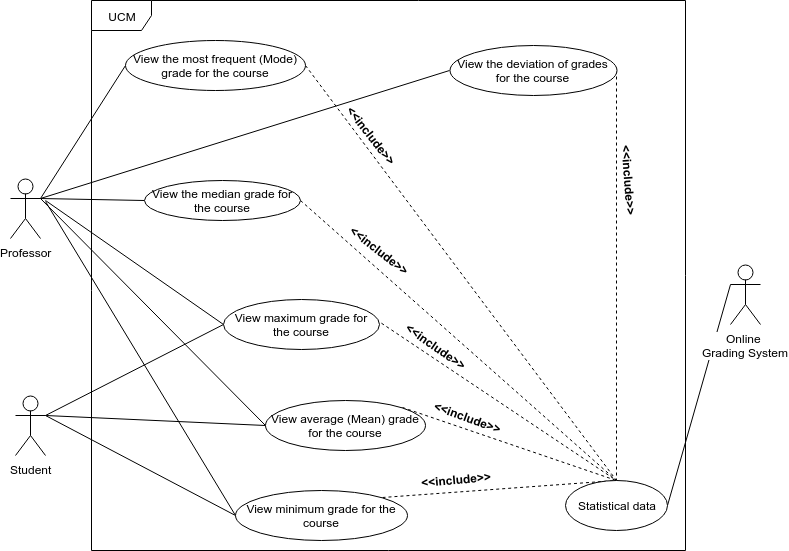
\includegraphics[width=\textwidth]{UCMv2.png}
\caption{Use case model}
\end{figure}
\newpage
\subsection{Use cases}

\begin{usecase}{View the most frequent (Mode) grade for the course}
    \addrow{Actors}{Professor, Online Grading System}
    \addrow{Precondition}{Professor has access to the system}
    \addrow{Postcondition}{Professor views the mode of grades}
    \addmulrow{Main scenario (M)}{
        \item Professor logins to the system
        \item System through statistical data module connects to the Online Grading System
        \item System shows the list of available courses
        \item Professor chooses the course to view
        \item System shows the statistics of the course
        \item Professor views the mode of course
    }
    \adddoublerow{Extensions (E)}{
        \item[] 1.1. Professor entered the wrong credentials
        \item[] 1.2. Go to 1
    }
\end{usecase}

\begin{usecase}{View the deviation of grades for the course}
    \addrow{Actors}{Professor, Online Grading System}
    \addrow{Precondition}{Professor has access to the system}
    \addrow{Postcondition}{Professor views the deviation of grades}
    \addmulrow{Main scenario (M)}{
        \item Professor logins to the system
        \item System through statistical data module connects to the Online Grading System
        \item System shows the list of available courses
        \item Professor chooses the course to view
        \item System shows the statistics of the course
        \item Professor views the deviation of grades
    }
    \adddoublerow{Extensions (E)}{
        \item[] 1.1. Professor entered the wrong credentials
        \item[] 1.2. Go to 1
    }
\end{usecase}
\newpage
\begin{usecase}{View the median grade for the course}
    \addrow{Actors}{Professor, Online Grading System}
    \addrow{Precondition}{Professor has access to the system}
    \addrow{Postcondition}{Professor views the median grade}
    \addmulrow{Main scenario (M)}{
        \item Professor logins to the system
        \item System through statistical data module connects to the Online Grading System
        \item System shows the list of available courses
        \item Professor chooses the course to view
        \item System shows the statistics of the course
        \item Professor views the median grade
    }
    \adddoublerow{Extensions (E)}{
        \item[] 1.1. Professor entered the wrong credentials
        \item[] 1.2. Go to 1
    }
\end{usecase}

\begin{usecase}{View average (Mean) grade for the course}
    \addrow{Actors}{Professor, Student, Online Grading System}
    \addrow{Precondition}{Professor has access to the system. Student has access to the system}
    \addrow{Postcondition}{Professor views average (Mean) grade. Student views average (Mean) grade.}
    \addmulrow{Main scenario (M)}{
        \item Professor or Student logins to the system
        \item System through statistical data module connects to the Online Grading System
        \item System shows the list of available courses for the user (Professor or Student)
        \item Professor or Student chooses the desirable course
        \item System shows the average (Mean) grade for the course
    }
    \adddoublerow{Extensions (E)}{
        \item[] 1.1. Professor or Student entered the wrong credentials
        \item[] 1.2. Go to 1
    }
\end{usecase}
\newpage
\begin{usecase}{View minimum grade for the course}
    \addrow{Actors}{Professor, Student, Online Grading System}
    \addrow{Precondition}{Professor has access to the system. Student has access to the system}
    \addrow{Postcondition}{Professor views minimum grade. Student views minimum grade.}
    \addmulrow{Main scenario (M)}{
        \item Professor or Student logins to the system
        \item System through statistical data module connects to the Online Grading System
        \item System shows the list of available courses for the user (Professor or Student)
        \item Professor or Student chooses the desirable course
        \item System shows the minimum grade for the course
    }
    \adddoublerow{Extensions (E)}{
        \item[] 1.1. Professor or Student entered the wrong credentials
        \item[] 1.2. Go to 1
    }
\end{usecase}

\begin{usecase}{View maximum grade for the course}
    \addrow{Actors}{Professor, Student, Online Grading System}
    \addrow{Precondition}{Professor has access to the system. Student has access to the system}
    \addrow{Postcondition}{Professor views maximum grade. Student views maximum grade.}
    \addmulrow{Main scenario (M)}{
        \item Professor or Student logins to the system
        \item System through statistical data module connects to the Online Grading System
        \item System shows the list of available courses for the user (Professor or Student)
        \item Professor or Student chooses the desirable course
        \item System shows the maximum grade for the course
    }
    \adddoublerow{Extensions (E)}{
        \item[] 1.1. Professor or Student entered the wrong credentials
        \item[] 1.2. Go to 1
    }
\end{usecase}
%-----------------------------------------------------------------
\section{Part - Estimates of effort}
\subsection{UCP}
The \textbf{UCP} is effort estimation approach. To calculate effort there are number of needed equations: \textbf{UUCP} (Unadjusted Use Case Points), \textbf{TCF} (Technical Complexity Factor), \textbf{ECF} (Environment Complexity Factor). \\
\begin{equation}
    \textbf{UCP} = \textbf{UUCP} \times \textbf{TCF} \times \textbf{ECF}
\end{equation}\\

The \textbf{UUCP} based on the sum of \textbf{UAW} (Unadjusted Actor Weight)
and \textbf{UUCW} (Unadjusted Use Case Weight).\\
\begin{equation}
    \textbf{UUCP} = \textbf{UAW} + \textbf{UUCW}
\end{equation}\\

The \textbf{UAW} based on the aggregated complexity of all the actors in all the use cases.
\begin{equation}
    \textbf{UAW} = \sum^{}_{}{Actors * Weight}
\end{equation}\\
\begin{table}[h]
\centering
\caption{The classification of actors and their associated weights in the UCP approach.}
\begin{tabular}{|l|l|l|}
\hline
\textbf{Actor type} & \textbf{Description} & \textbf{Weight} \\ \hline
A1                  & Simple actor         & 1               \\ \hline
A2                  & Average actor        & 2               \\ \hline
A3                  & Complex actor        & 3               \\ \hline
\end{tabular}
\end{table}
Based on the \textbf{UCM} we have 2 complex actors and 1 simple, then:
\begin{equation}
    \textbf{UAW} = 1\times3 + 1\times3 + 1\times1
\end{equation}
\begin{equation}
    \textbf{UAW} = 7
\end{equation}\\

the \textbf{UUCW} is based on the total number of steps contained in all the use case scenarios.
\begin{equation}
    \textbf{UUCW} = \sum^{}_{}{UseCase * Weight}
\end{equation}\\
\begin{table}[h]
\centering
\caption{shows that there are 3 types of use cases, each assigned a weight. }
\begin{tabular}{|l|l|l|}
\hline
\textbf{Use Case Type} & \textbf{Description} & \textbf{Weight} \\ \hline
UC1                    & Simple Use Case      & 5               \\ \hline
UC2                    & Average Use Case     & 10              \\ \hline
UC3                    & Complex Use Case     & 15              \\ \hline
\end{tabular}
\end{table}
Based on the \textbf{UCM} we have 6 simple use cases, then:
\begin{equation}
    \textbf{UUCW} = 6 \times 5
\end{equation}
\begin{equation}
    \textbf{UUCW} = 30
\end{equation}\\

In this case the \textbf{UUCP} is:
\begin{equation}
    \textbf{UUCP} = 7 + 30
\end{equation}
\begin{equation}
    \textbf{UUCP} = 37
\end{equation}\\

The purpose of \textbf{TCF} (Technical complexity factor) is to account for the technical concerns that can impact the software project from its inception to its conclusion, including delivery.
\begin{equation}
    \textbf{TCF} = C1 + \Bigg[C2 \times \sum^{13}_{i=1}{(W_{Ti} \times F_{i})\Bigg]} 
\end{equation}\\
Where $C1 = 0.6$, $C2 = 0.01$, $W_{Ti}$ is the Technical Complexity Factor Weight, and $F_{i}$ is the Perceived Impact Factor corresponding to each Technical Complexity Factor. 

\begin{table}[h]
\centering
\caption{The Technical Complexity Factors in the UCP approach.}
\begin{tabular}{|l|l|l|l|}
\hline
\multicolumn{1}{|c|}{\textbf{TCF Type}} & \multicolumn{1}{c|}{\textbf{Description}} & \multicolumn{1}{c|}{\textbf{Weight}} & \multicolumn{1}{c|}{\textbf{Factor}} \\ \hline
T1 & Distributed System & 2 & 0 \\ \hline
T2 & Performance & 1 & 5 \\ \hline
T3 & End User Efficiency & 1 & 4 \\ \hline
T4 & Complex Internal Processing & 1 & 3 \\ \hline
T5 & Reusability & 1 & 5 \\ \hline
T6 & Easy to Install & 0.5 & 4 \\ \hline
T7 & Easy to Use & 0.5 & 5 \\ \hline
T8 & Portability & 2 & 5 \\ \hline
T9 & Easy to Change & 1 & 5 \\ \hline
T10 & Concurrency & 1 & 4 \\ \hline
T11 & Special Security Features & 1 & 0 \\ \hline
T12 & Provides Direct Access for Third Parties & 1 & 0 \\ \hline
T13 & Special User Training Facilities are Required & 1 & 0 \\ \hline
\end{tabular}
\end{table}
In this case the \textbf{TCF} is:
\begin{equation}
    \textbf{TCF} =  0.6 + \Big[0.01 \times(2\times0+1\times5+1\times4+1\times3+1\times5+0.5\times4+0.5\times5+2\times5+1\times5+1\times4+1\times0+1\times0+1\times0)\Big]
\end{equation}
\begin{equation}
    \textbf{TCF} =  1.005
\end{equation}\\
\newpage
The purpose of \textbf{ECF} is to account for the development team's personal traits, including experience.
\begin{equation}
    \textbf{ECF} = C1 + \Bigg[C2 \times \sum^{8}_{i=1}{(W_{Ei} \times F_{i})\Bigg]} 
\end{equation}\\
Where $C1 = 1.4$, $C2 = - 0.03$, $W_{Ei}$ is the Environmental Complexity Factor Weight, and $F_{i}$ is the Perceived Impact Factor corresponding to each Environmental Complexity Factor.

\begin{table}[h]
\centering
\caption{The Environmental Complexity Factors in the UCP approach.}
\begin{tabular}{|l|l|l|l|}
\hline
\multicolumn{1}{|c|}{\textbf{ECF Type}} & \multicolumn{1}{c|}{\textbf{Description}} & \multicolumn{1}{c|}{\textbf{Weight}} & \multicolumn{1}{c|}{\textbf{Factor}} \\ \hline
E1 & Familiarity with the Use Case Domain & 1.5 & 4 \\ \hline
E2 & Part-Time Workers & -1 & 3 \\ \hline
E3 & Analyst Capability & 0.5 & 3 \\ \hline
E4 & Application Experience & 0.5 & 4 \\ \hline
E5 & Object-Oriented Experience & 1 & 5 \\ \hline
E6 & Motivation & 1 & 5 \\ \hline
E7 & Difficult Programming Language & -1 & 5 \\ \hline
E8 & Stable Requirements & 2 & 5 \\ \hline
\end{tabular}
\end{table}

In this case the \textbf{ECF} is:
\begin{equation}
    \textbf{ECF} =  1.4 + \Big[-0.03 \times(1.5\times4+(-1\times3)+0.5\times3+0.5\times4+1\times5+1\times5+(-1\times5)+2\times5)\Big]
\end{equation}
\begin{equation}
    \textbf{ECF} =  0.755
\end{equation}\\

The \textbf{UCP} is equal:
\begin{equation}
    \textbf{UCP} = 37 \times 1.005 \times 0.755
\end{equation}
\begin{equation}
    \textbf{UCP} = 28.075
\end{equation}\\

Since the team is new, the \textbf{PF} (Productivity Factor) is equal 20.
In this case the Effort Estimate is:
\begin{equation}
    \textbf{Effort Estimate} = \textbf{UCP} \times \textbf{PF}
\end{equation}
\begin{equation}
    \textbf{Effort Estimate} = 28.075 \times 20
\end{equation}
\begin{equation}
    \textbf{Effort Estimate} = 561.5 \quad \textrm{person-hours} \quad
\end{equation}\\

Therefore, the estimated effort of the project by using \textbf{UCP} method is \textbf{562} person-hours.

\subsection{COCOMO 81}
hello world
\subsection{Difference in estimates using UCP and COCOMO 81}
hello world

%-----------------------------------------------------------------
\section{Part - Implementation}
\subsection{Code listings}
The code listing of implemented functions.
\subsubsection{Min function}

\begin{lstlisting}[language=R]
min <- function(array){
  res <- 9999999999999999
  for(elem in array){
    if(elem < res){
      res <- elem
    }
  }
  return(res)
}
\end{lstlisting}

\subsubsection{Max function}

\begin{lstlisting}[language=R]
max <- function(array){
  res <- -9999999999999999
  for(elem in array){
    if(elem > res){
      res <- elem
    }
  }
  return(res)
}
\end{lstlisting}
\subsection{Testing}

%-----------------------------------------------------------------
\section{Part - Cyclomatic complexity}

%-----------------------------------------------------------------
\section{Part - Object-oriented metrics}

%-----------------------------------------------------------------
\section{Part - SLOC}

%-----------------------------------------------------------------
\section{{Part - Correlations}}

%-----------------------------------------------------------------
%Don't delete below
\bibliography{ref}{}
\bibliographystyle{plain}
\end{document}               % End of document.